\mode*

% Since this a solution template for a generic talk, very little can
% be said about how it should be structured. However, the talk length
% of between 15min and 45min and the theme suggest that you stick to
% the following rules:  

% - Exactly two or three sections (other than the summary).
% - At *most* three subsections per section.
% - Talk about 30s to 2min per frame. So there should be between about
%   15 and 30 frames, all told.


\section{One-way functions}

\subsection{Hash functions}

\begin{frame}
  \begin{idea}
    \begin{itemize}
      \item We want a function which we can efficiently compute.
      \item However, it shouldn't be possible to find its inverse.
    \end{itemize}
  \end{idea}

  \pause{}

  \begin{example}
    \begin{description}
      \item[Easy] \(f(x) = y\)
      \item[Hard] \(f^{-1}(y) = x\)
    \end{description}
  \end{example}
\end{frame}

\begin{frame}
  \begin{figure}
    \subfloat[\(h\colon X\to Y\)]{%
      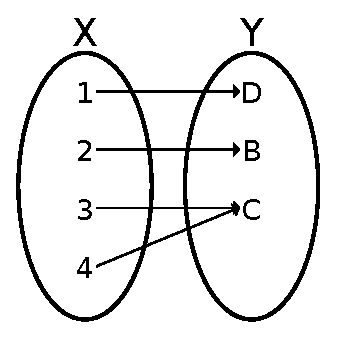
\includegraphics[height=2cm]{surjection.eps}%
    }
    \hspace{0.1\textwidth}
    \subfloat[\(h^\prime\colon X\to Y\)]{%
      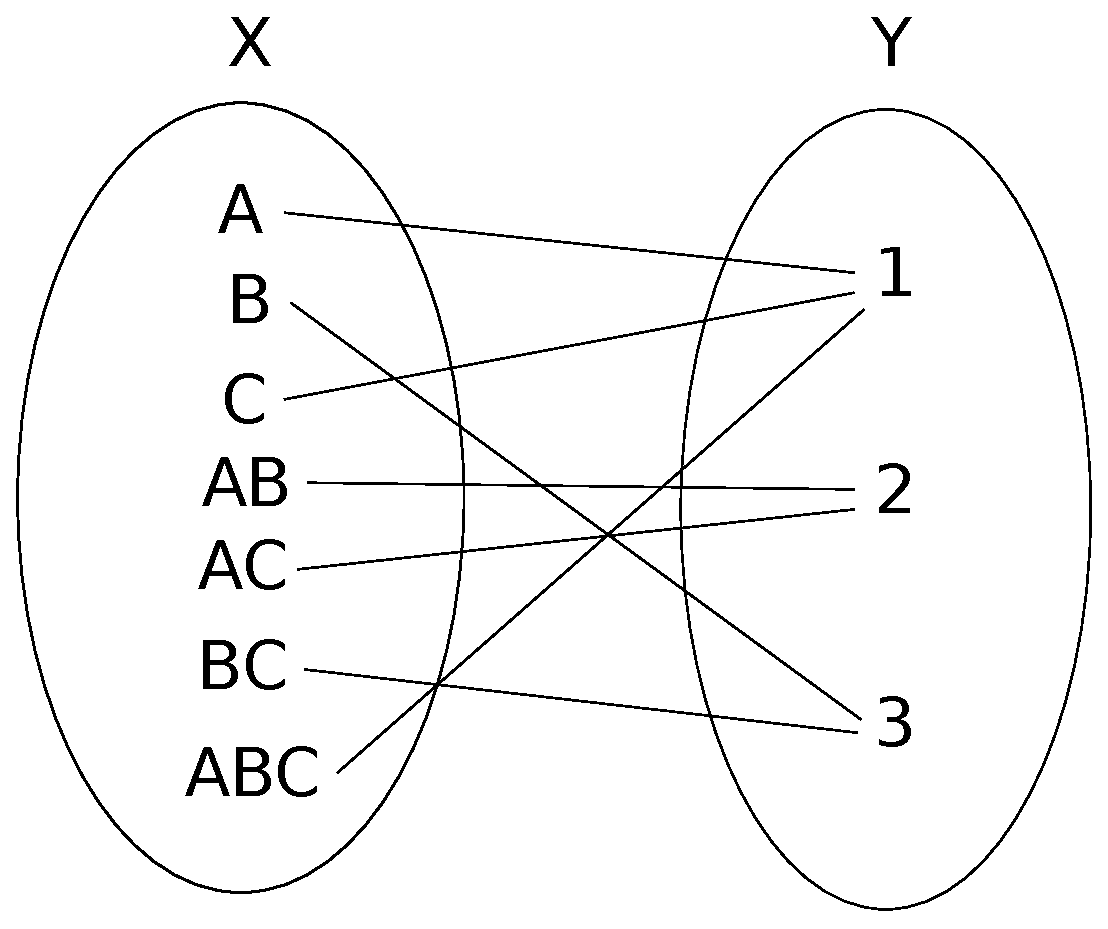
\includegraphics[height=2cm]{hashfunc.eps}%
    }
    \caption{%
      Two non-injective, surjective functions \(h\) and \(h^\prime\).
    }
  \end{figure}

  \begin{exercise}
    Could either of these two functions be one-way functions?
  \end{exercise}
\end{frame}

\begin{frame}
  \begin{definition}[One-way function\footfullcite{GoldreichFOC-1}]
    \begin{itemize}
      \item Let \(h\colon \{0,1\}^*\to \{0,1\}^*\).
      \item \(h\) is \emph{one-way} if
        \begin{enumerate}
          \item there exists an efficient algorithm \(A\) such that \(A(x) 
              = h(x)\);
          \item for every efficient algorithm \(A^\prime\), every positive 
            polynomial \(p(\cdot)\) and all sufficiently large \(n\)'s
            \[\Prob{A^\prime(h(x), 1^n) \in h^{-1}(h(x))} < \frac{1}{p(n)}\]
        \end{enumerate}
    \end{itemize}
  \end{definition}
\end{frame}

\begin{frame}
  \begin{example}[Implementations you might've heard of]
    \begin{itemize}
      \item MD5
      \item SHA1
      \item SHA256 (SHA-2)
      \item SHA-3
    \end{itemize}
  \end{example}
  \begin{example}[Applications]
    \begin{itemize}
      \item Verifying file content integrity
      \item Digital signatures
      \item Protect passwords
    \end{itemize}
  \end{example}
\end{frame}

\begin{frame}
  \begin{remark}
    \begin{itemize}
      \item One-wayness returns as a useful property in many situations.
      \item Encryption also has the one-wayness property:
        \begin{description}
          \item[Easy] Given \(k, m\), compute \(c\gets \Enc[_k][m]\).
          \item[Hard] Given \(c\), compute either of \(k, m\).
        \end{description}
      \item However, encryption is bijective, hash functions are generally not.
    \end{itemize}
  \end{remark}
\end{frame}

\subsection{\Aclp{MAC}}

\begin{frame}
  \begin{example}
    \begin{itemize}
      \item Let \(\Enc[_k][\cdot] = \Dec[_k][\cdot] = \cdot\oplus k\bmod 2\).
        
        \pause{}

      \item Alice and Bob share \(k\).
      \item Alice sends \(\Enc[_k][m] = c\) to Bob.

        \pause{}

      \item Eve intercepts \(c\), she cannot get to \(m\).

        \pause{}

      \item Eve computes \(c' = c\oplus m_E\) and passes \(c'\) to Bob.

        \pause{}

      \item Bob computes \(\Dec[_k][c'] = \Dec[_k][c\oplus m_E] = m\oplus 
        k\oplus m_E\oplus k = m\oplus m_E\).
    \end{itemize}
  \end{example}

  \pause{}
  
  \begin{exercise}
    How can we solve this?
    Bob needs to know that Eve modified the message!
  \end{exercise}
\end{frame}

\begin{frame}
  \begin{idea}[\acp{MAC}]
    \acuse{MA}
    \begin{itemize}
      \item Alice and Bob need something that Eve doesn't know how to modify.

        \pause{}

      \item If that something is tied to the message, then a modified message 
        would be detectable.
    \end{itemize}
  \end{idea}

  \pause{}

  \begin{exercise}
    Any ideas on how we can construct such a thing?
  \end{exercise}
\end{frame}

\begin{frame}
  \begin{example}
    \begin{itemize}
      \item Let \(h\) be a one-way function.
        
        \pause{}
        
      \item If we use \(h(c) = t\), then Eve can also compute the hash 
        function: \(h(c^\prime) = t^\prime\).

        \pause{}

      \item A secret hash function would violate Kerckhoff's principle, so 
        that's not an option.

        \pause{}

      \item If we instead use the message, rather than the ciphertext.
        
      \item Then \(h(m) = t\) and
        \begin{itemize}
          \item \(\Dec[k]{c^\prime} = m^\prime = m\oplus m_E, h(m^\prime)\neq 
              t\).
          \item \(\Dec[k]{c} = m, h(m) = t\).
        \end{itemize}

        \pause{}
        
      \item Eve makes up \(m'\), she can compute \(t' = h(m')\).
    \end{itemize}
  \end{example}
\end{frame}

\begin{frame}
  \begin{solution}
    \begin{itemize}
      \item Let \(s\) be a secret shared between Alice and Bob.

        \pause{}

      \item \(h(c\concat s) = t\), Eve doesn't know \(s\).
      \item Bob can immediately check \(h(c^\prime\concat s)\neq t\).
    \end{itemize}
  \end{solution}

  \pause{}

  \begin{remark}
    \begin{itemize}
      \item It requires even a bit more than this!
      \item But the idea is correct.
    \end{itemize}
  \end{remark}
\end{frame}

\begin{frame}
  \begin{solution}[\Acl{HMAC}, \acs{HMAC}\footfullcite{HMAC}]
    \begin{itemize}
      \item Let \(h\) be a one-way function.
      \item Let \(c\) be the ciphertext, \(s\) our \ac{MA} secret.

        \pause{}

      \item Then tag \(t = \HMAC[_s][c]\), where \[
          \HMAC[_s][c] = h\left[
            (s\oplus p_o)\concat h\left[ (s\oplus p_i)\concat c \right]
          \right],
        \] and \(p_i, p_o\) are inner and outer pads, respectively.
    \end{itemize}
  \end{solution}

  \pause{}

  \begin{remark}
    This is proven secure by \textcite{HMAC}!
  \end{remark}
\end{frame}

